\section{Systematic test}
\label{sec:swave:isobar}

The results shown in Figs.~\ref{fig:combods} and~\ref{fig:combofs} could
 have an implicit model dependence through the use of the LASS parametrisation to model the \psq spectrum.
 In order to understand the size of this effect, the measurements were repeated using an isobar
model to parametrise the \kpi S-wave as in Ref.~\cite{PhysRevLett.89.121801}.
In the isobar model the S-wave is described as a simple sum of functions for the $\Kstarzz(1430)$ 
and the $\kappa(800)$ along with a constant non-resonant term,
\begin{align}
T_I(\psq) &= N_{\kappa} \mathcal{F}_{\kappa}(\psq) \exp(\phi_{\kappa}) + N_S \mathcal{F}_S(\psq) \exp(\phi_S)  + NR
\end{align}
where $N_i$ is the normalisation for each contribution and $\phi_i$ is the phase of each contribution.
The $\Kstarzz(1430)$ is described by a relativistic Breit-Wigner function as in the LASS parametrisation,
\begin{align}
\mathcal{F}_S(\psq) &= \cot\delta_S = \frac{ \psq - m_{\mathrm{S}}^2 }{ \Gamma_{\mathrm{S}}(\psq) m_{\mathrm{S}}}.
\end{align}
and the $\kappa(800)$ is described similarly
\begin{align}
\mathcal{F}_{\kappa}(\psq) &= \cot\delta_{\kappa} = \frac{ \psq - m_{\kappa}^2 }{ \Gamma_{\kappa}(\psq) m_{\kappa}  }.
\end{align}
where the mass and width of the $\kappa(800)$ are taken from Ref.~\cite{PDG2012}.
The existence of the $\kappa(800)$ is under debate with no conclusive evidence.
The amplitude $T_I$ is normalised such that it has the same integral as the LASS amplitude ($T_S$) 
over the \psq range from threshold to an upper limit of 2.5\gevgevcccc. 
This limit is chosen to encompass most of resonant $\Kstarzz(1430)$.
The \psq spectrum of the combined P wave and the two S-wave models is shown in Fig.~\ref{fig:spwave:isobar}.
\begin{figure}[tb]
\centering
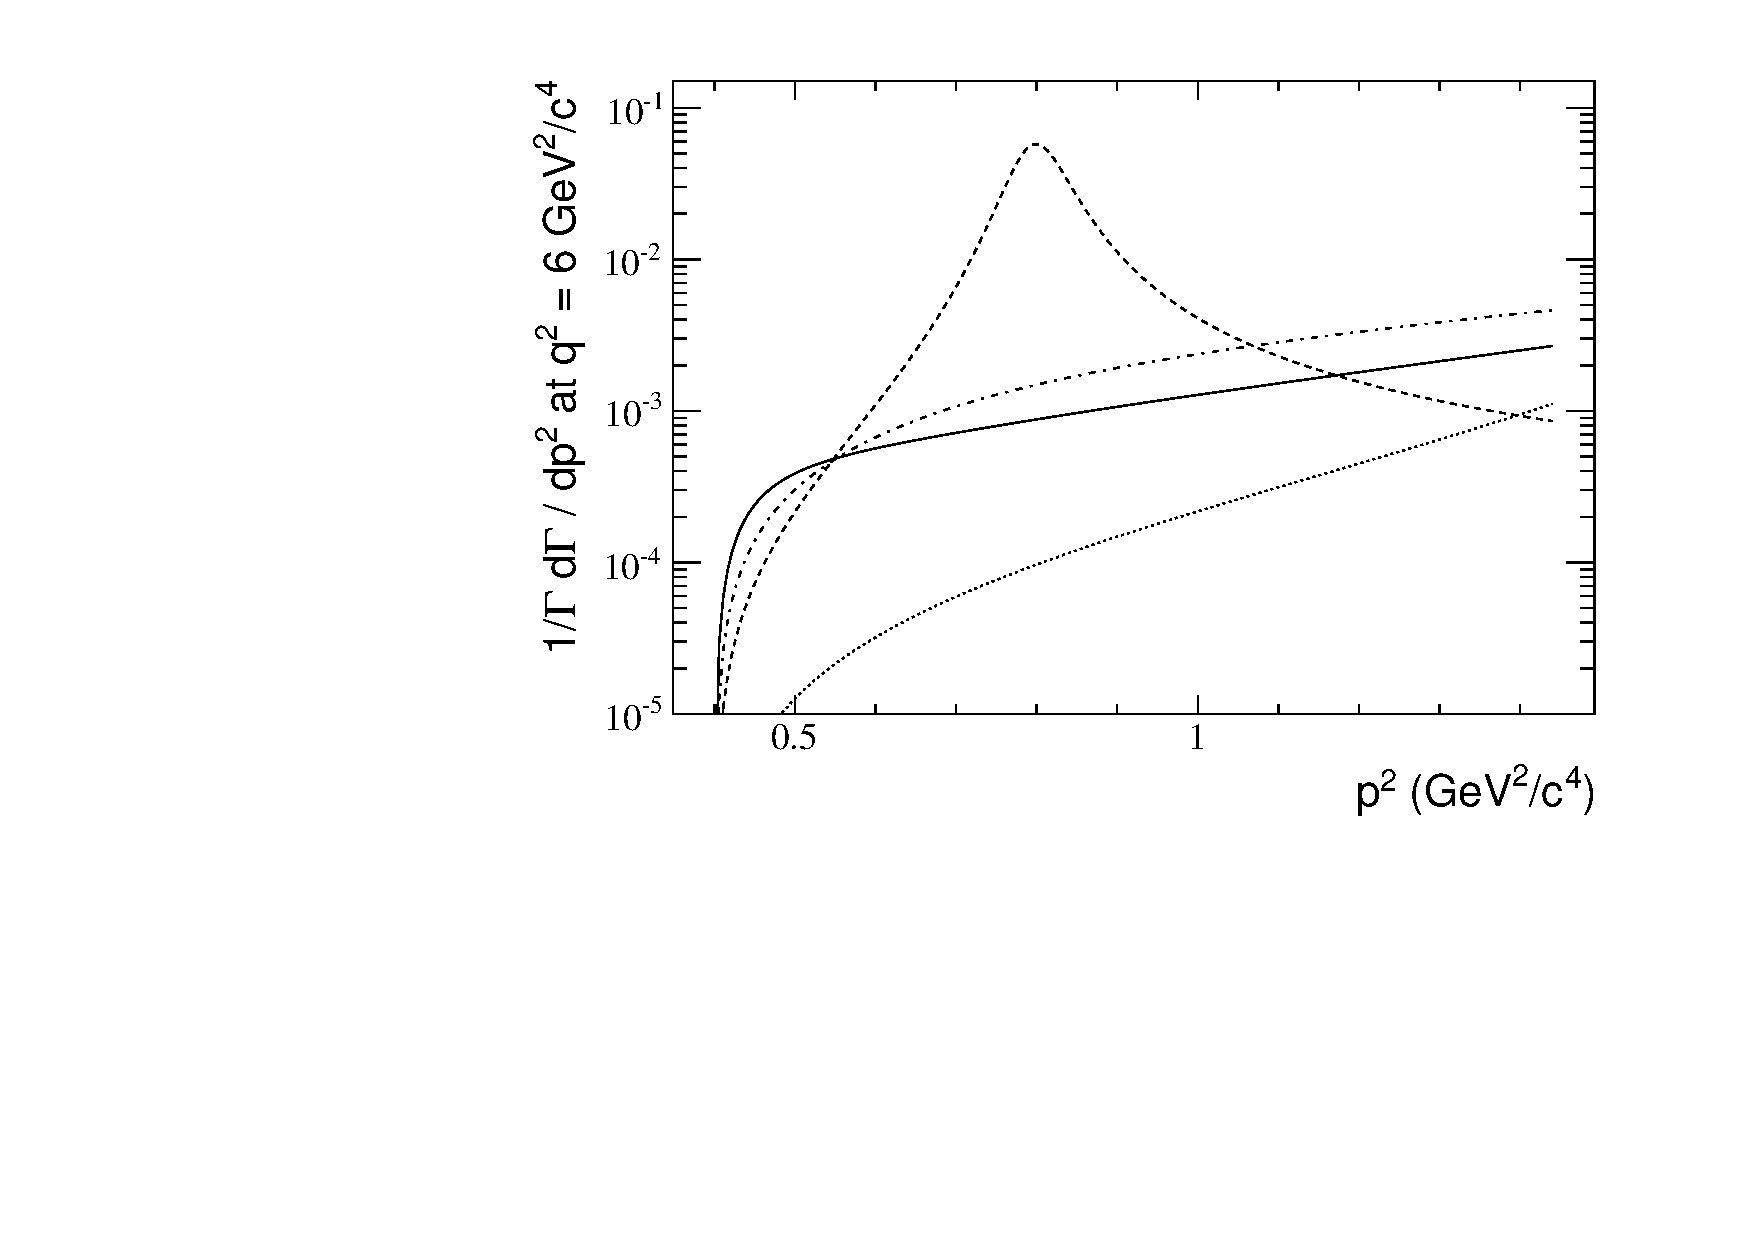
\includegraphics[width=0.66\textwidth]{chapter6/figs/calc_isobar_psq_branch_frac_logy.pdf}
\caption{ An illustration of the \psq spectrum for the P-wave (solid) and the
 isobar S-wave (dashed) and the LASS S-wave (dash-dotted) and the D-wave (dotted). 
~\label{fig:spwave:isobar} } 
\end{figure}

The model-dependence of the \psq spectrum was tested by generating events where an isobar model was used for 
the S-wave contribution and fitting the angular distribution using the LASS parametrisation.
The relative resolution between the results obtained when generating with the 
LASS parametrisation and the results obtained when generating with an isobar model
are shown in Fig.~\ref{fig:ratio:isobar}.
\begin{figure}[tb]
\centering
\subfigure[\AFB]{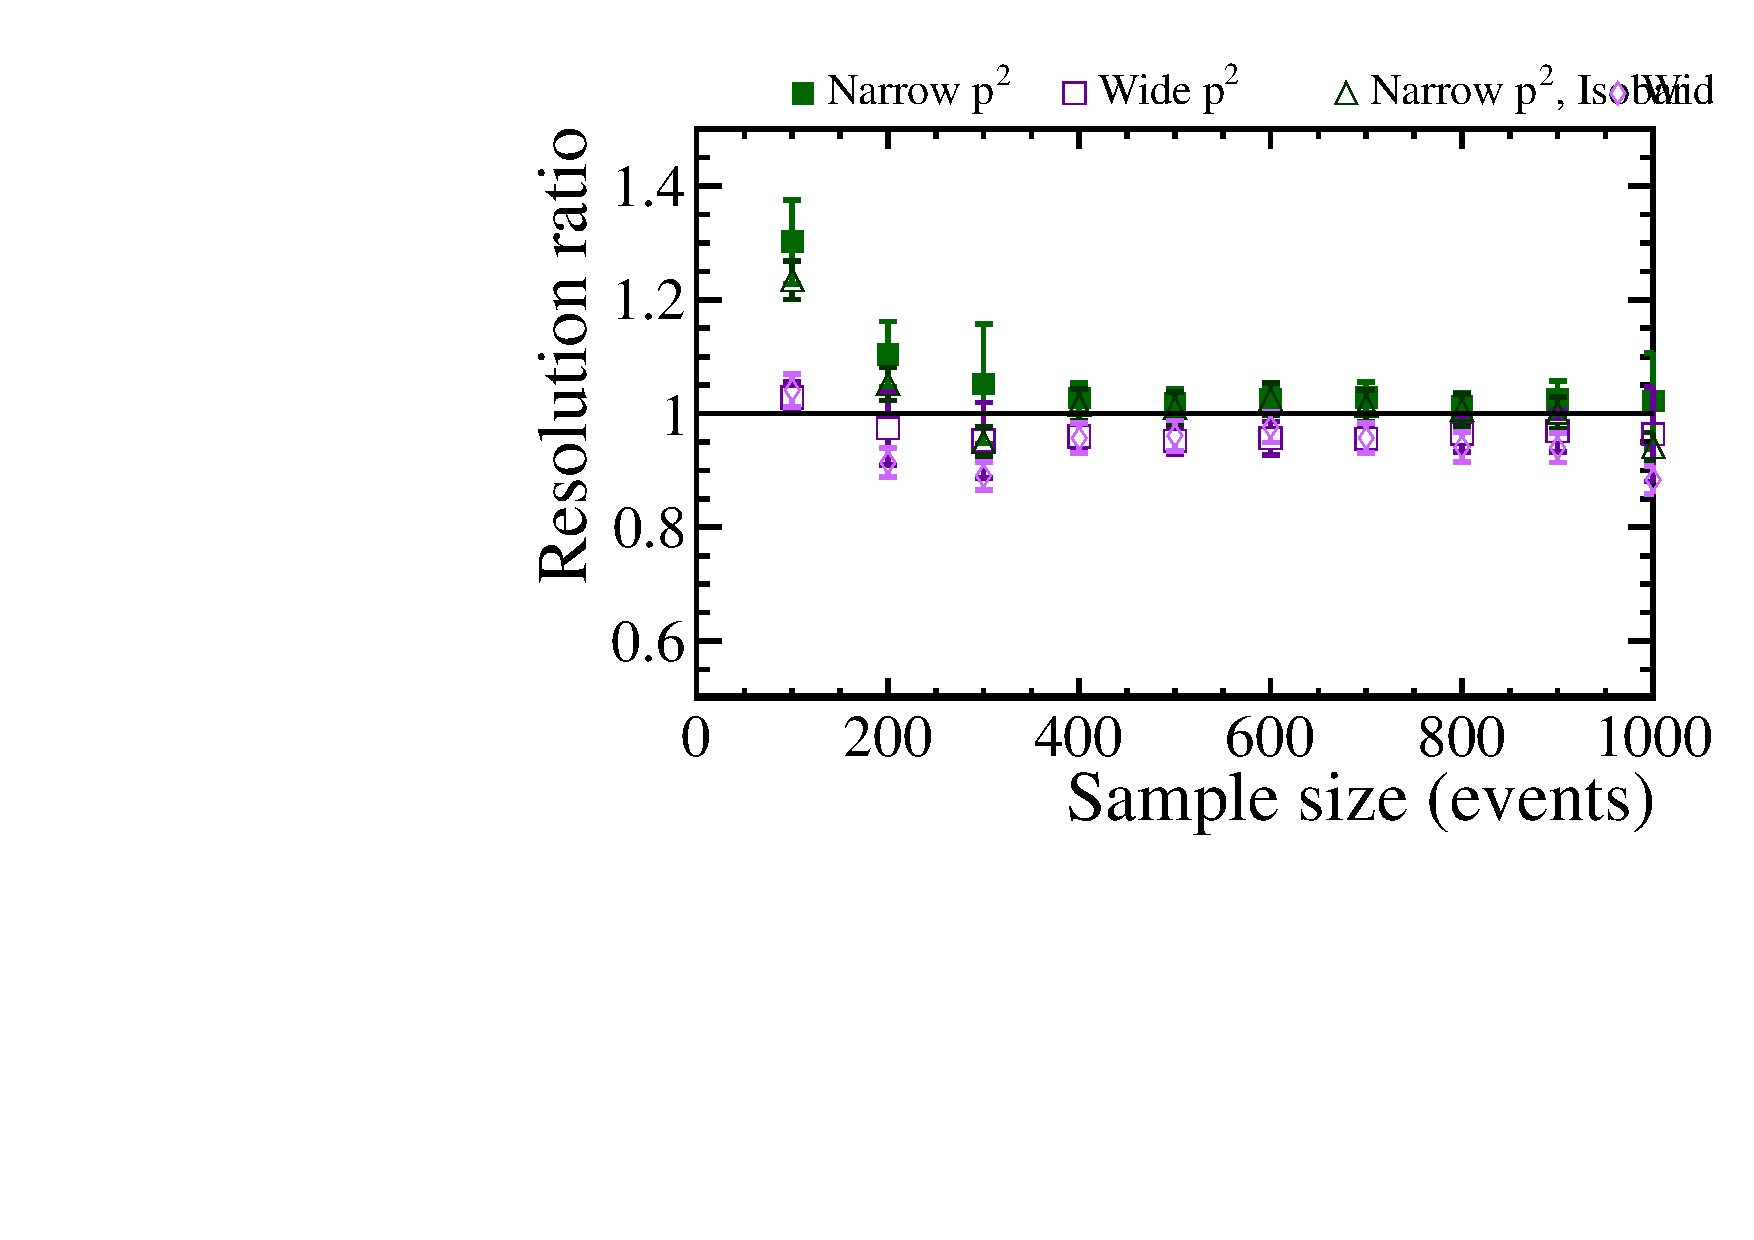
\includegraphics[width=0.48\textwidth]{chapter6/figs/fit_result_ratio_ds_isobar_afb_res.pdf}}
\subfigure[\FL]{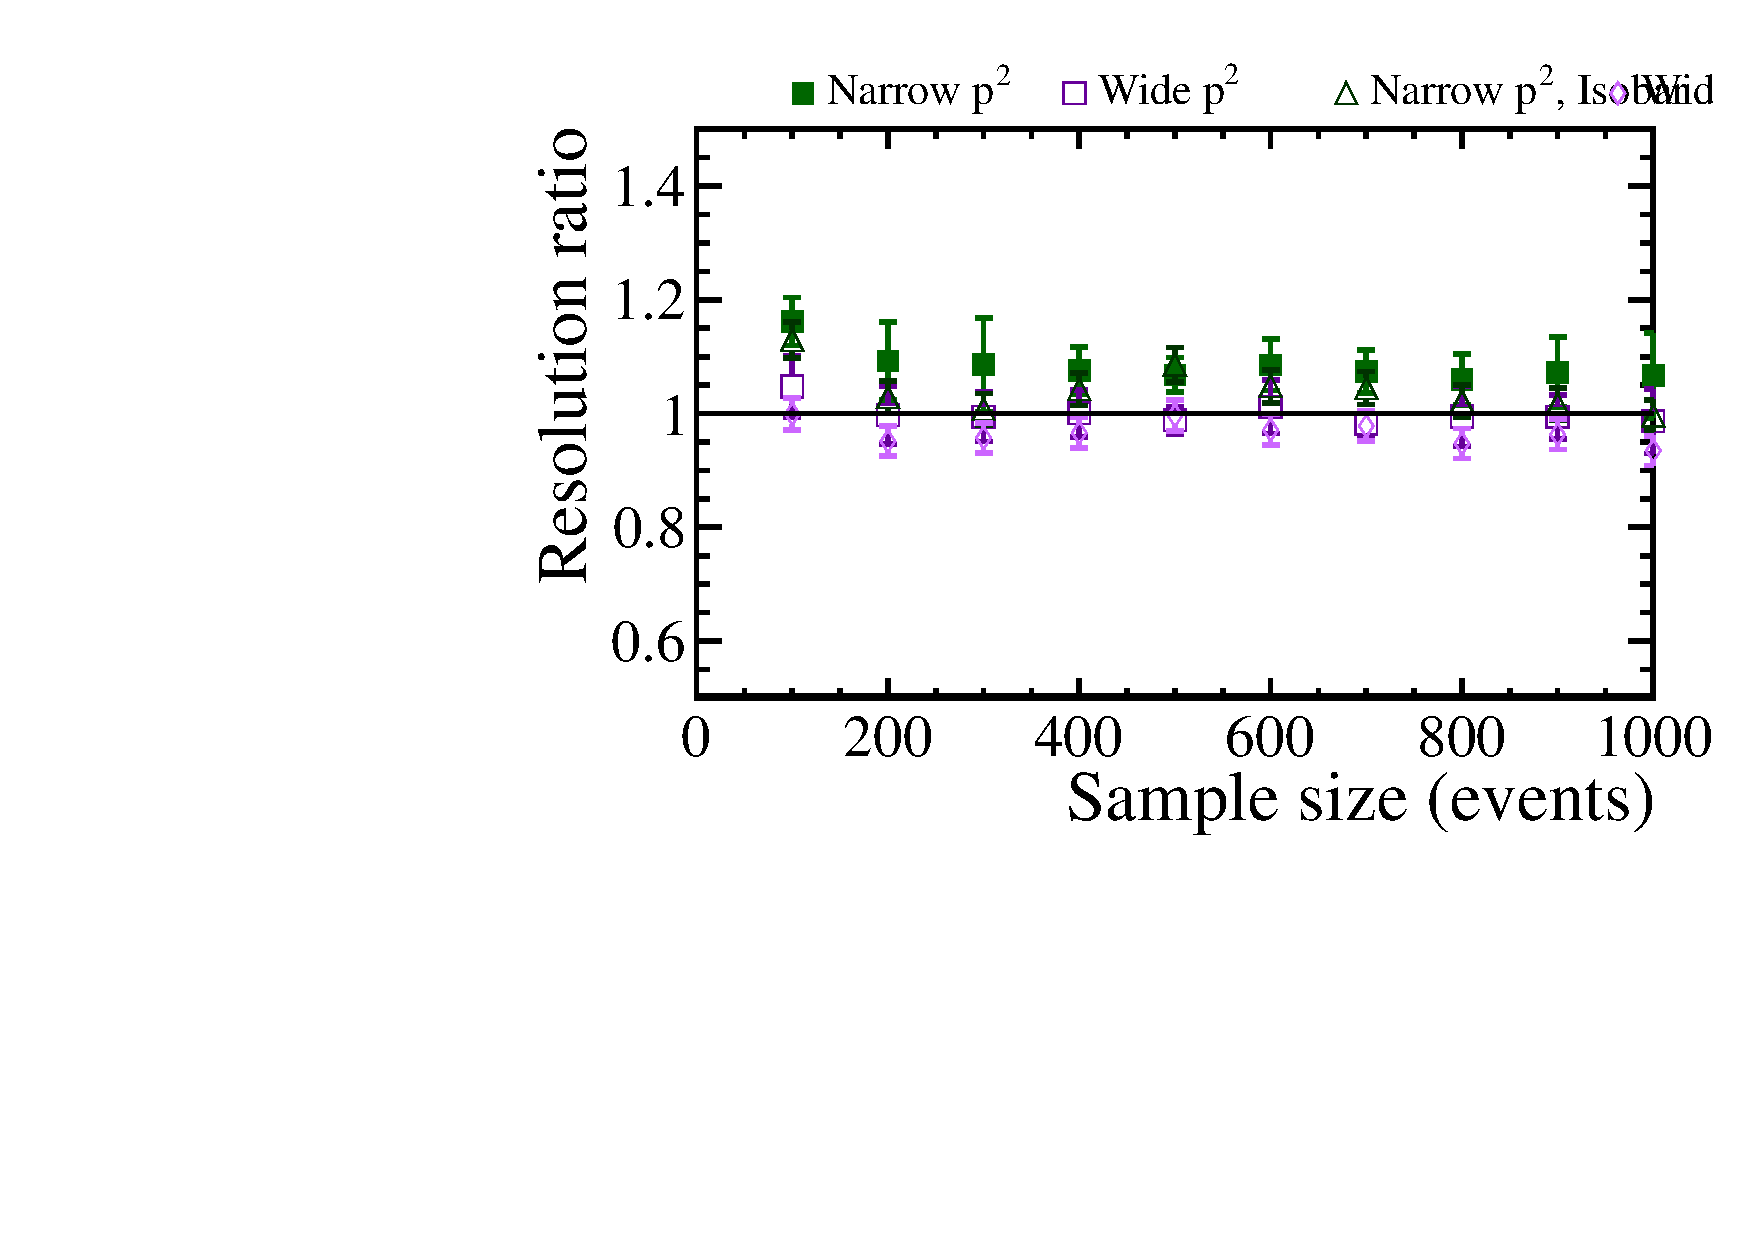
\includegraphics[width=0.48\textwidth]{chapter6/figs/fit_result_ratio_ds_isobar_fl_res.pdf}}
\subfigure[\AT2 ]{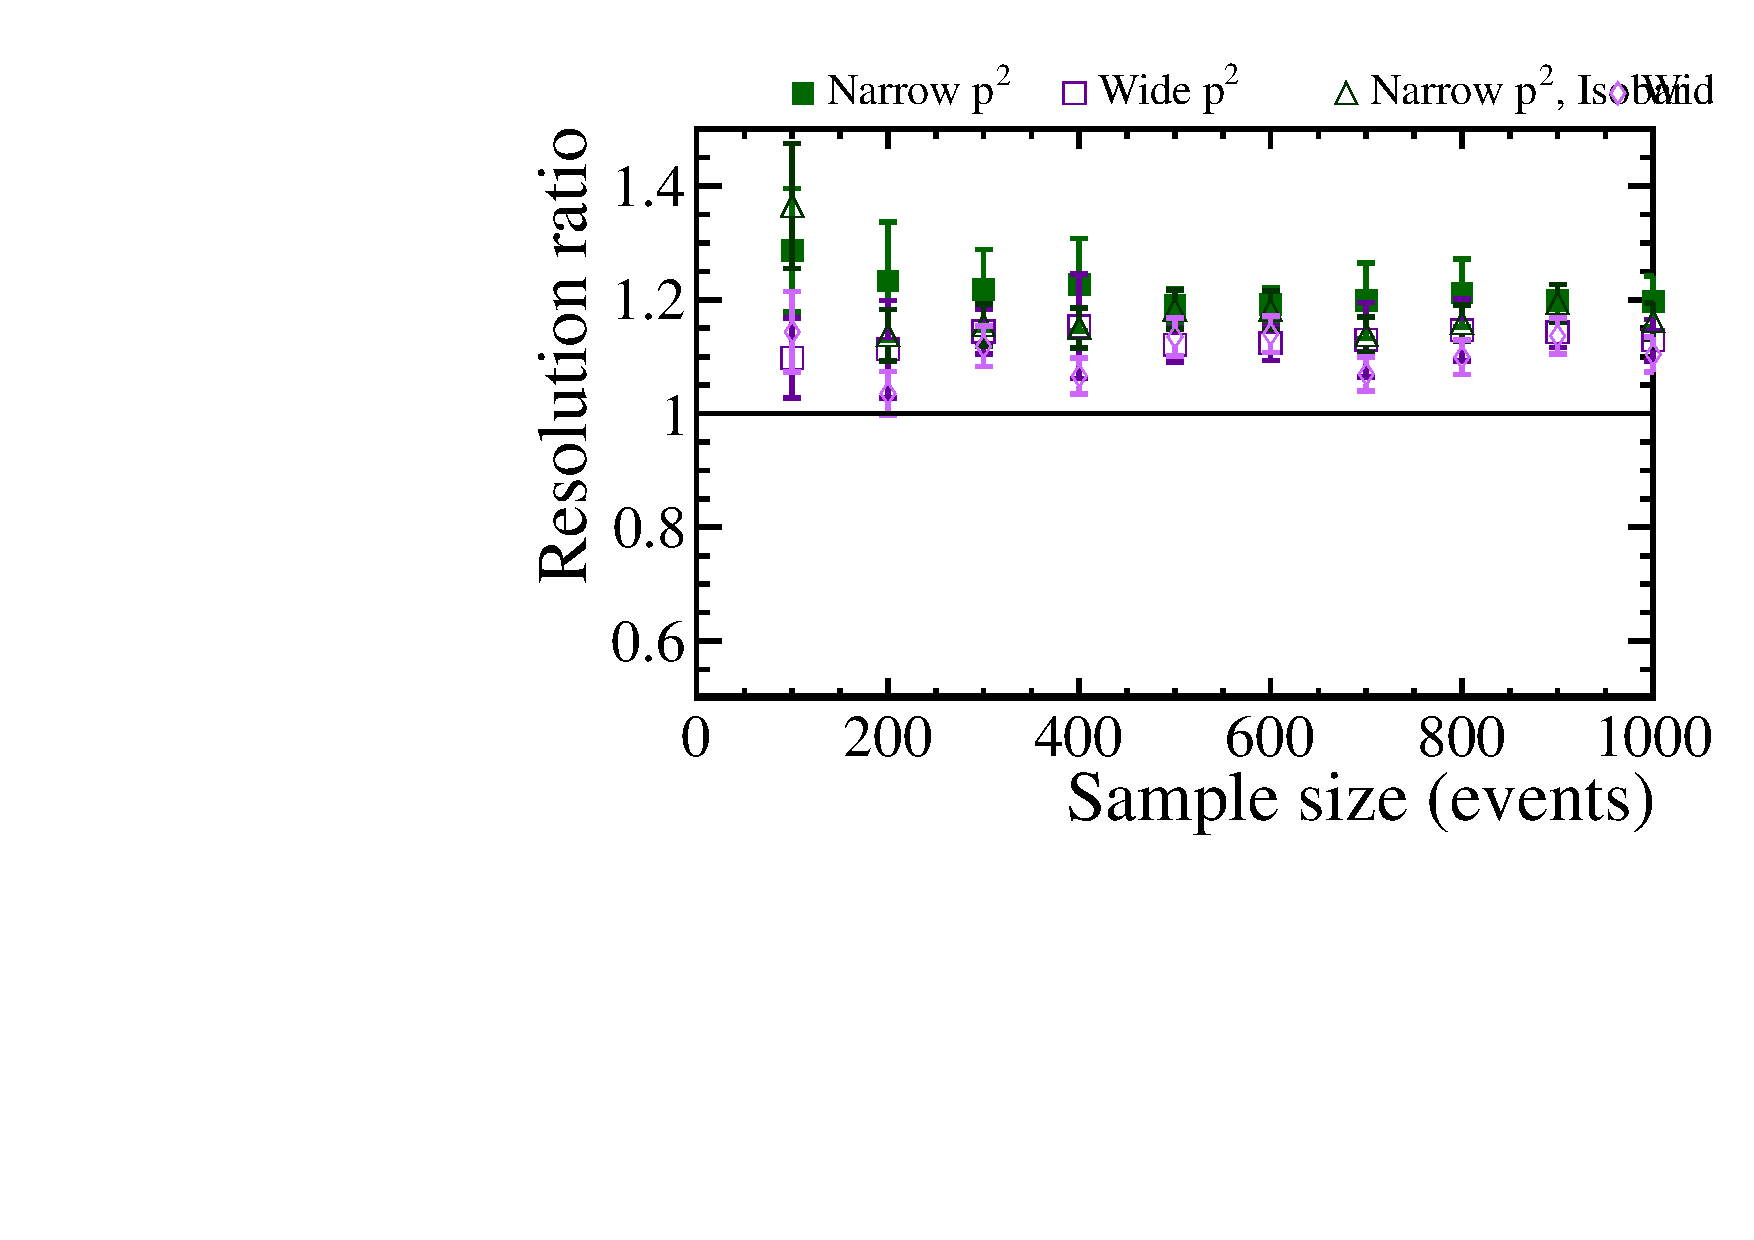
\includegraphics[width=0.48\textwidth]{chapter6/figs/fit_result_ratio_ds_isobar_at2_res.pdf}}
\subfigure[\AIm]{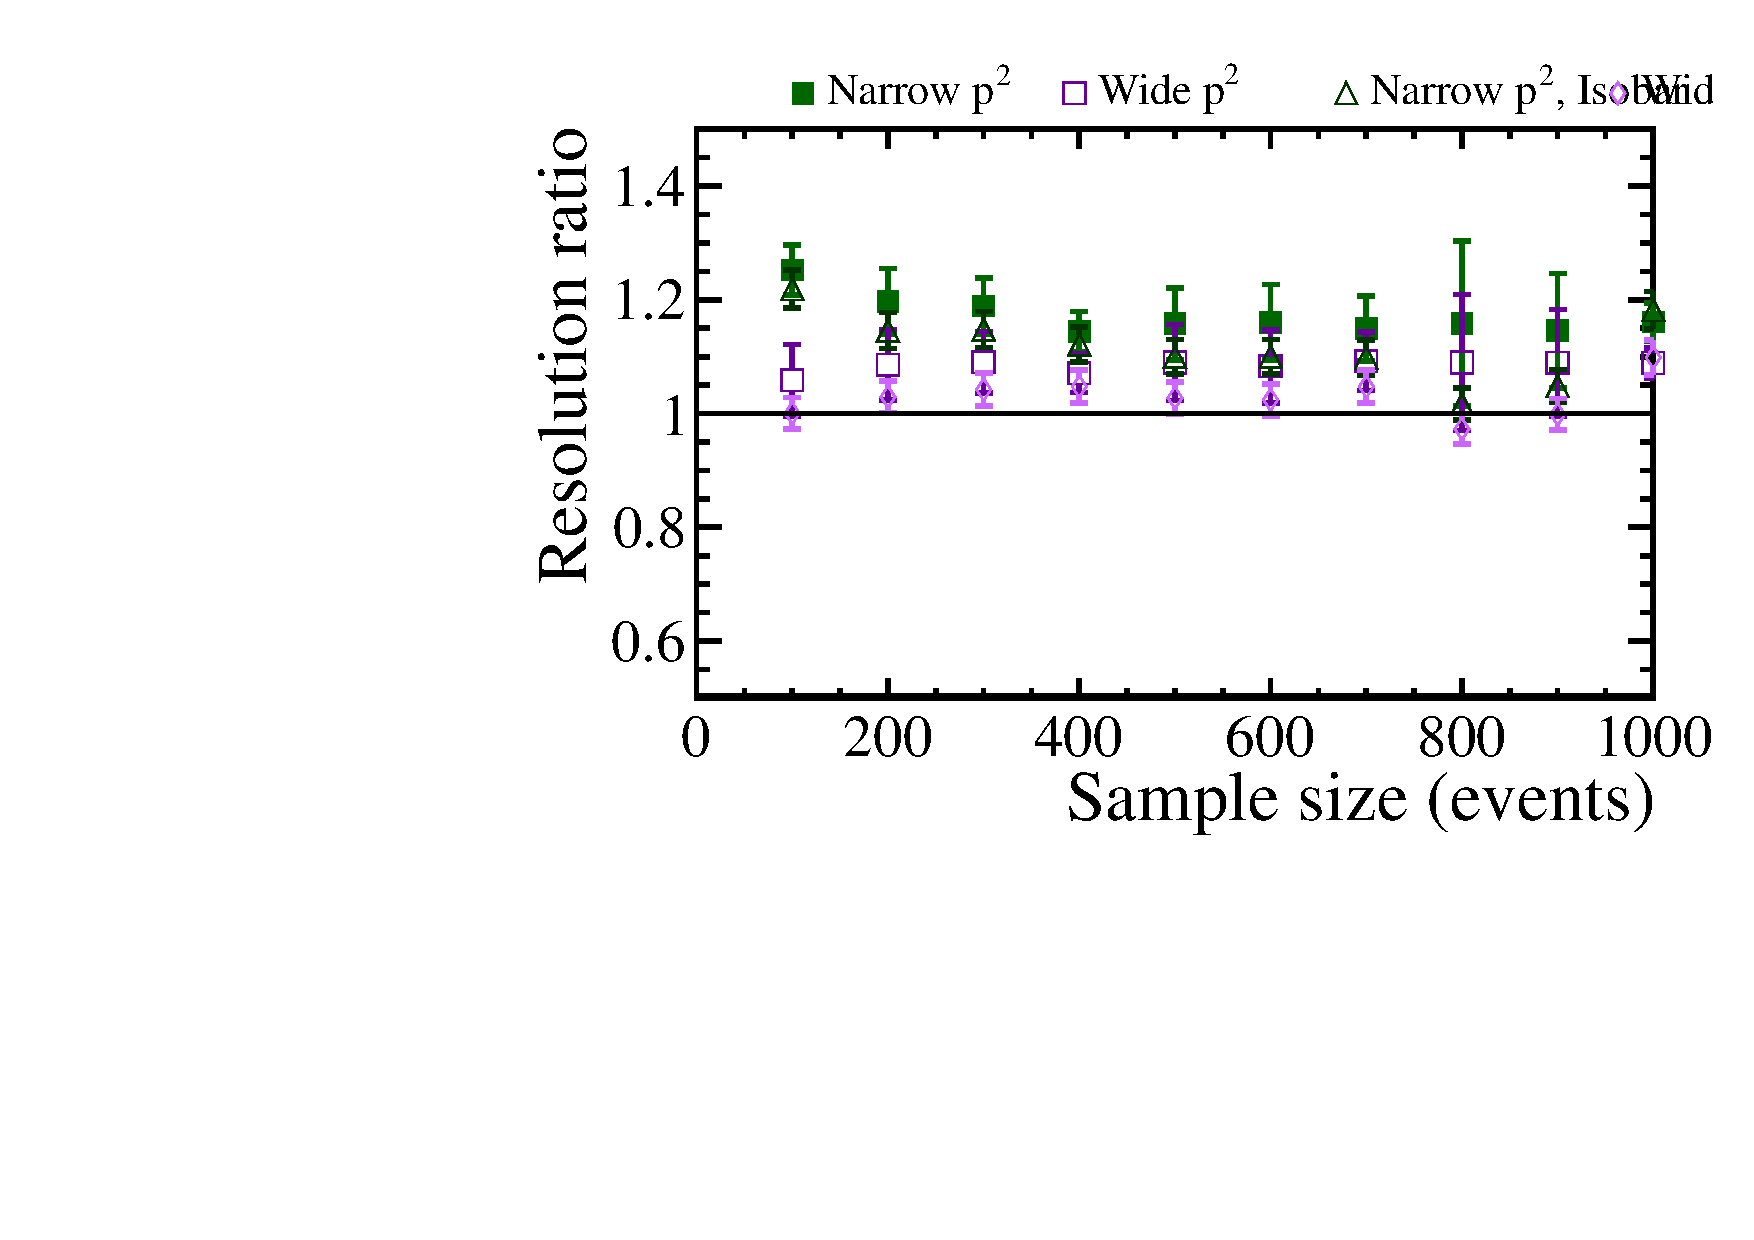
\includegraphics[width=0.48\textwidth]{chapter6/figs/fit_result_ratio_ds_isobar_aim_res.pdf}}
\caption[ Resolutions for three different methods to incorporate 
the S-wave relative to the resolution obtained when the S-wave is ignored.   ]
{Resolutions for three different methods to incorporate 
the S-wave relative to the resolution obtained when the S-wave is ignored. 
The S-wave has been generated using an isobar model. ~\label{fig:ratio:isobar}}
\end{figure}
The bias on the central values of the angular observables when the S-wave is ignored
as a function of the size of the dataset is shown in Fig.~\ref{fig:combods:isobar}.
\begin{figure}[tb]
\centering
\subfigure[\AFB]{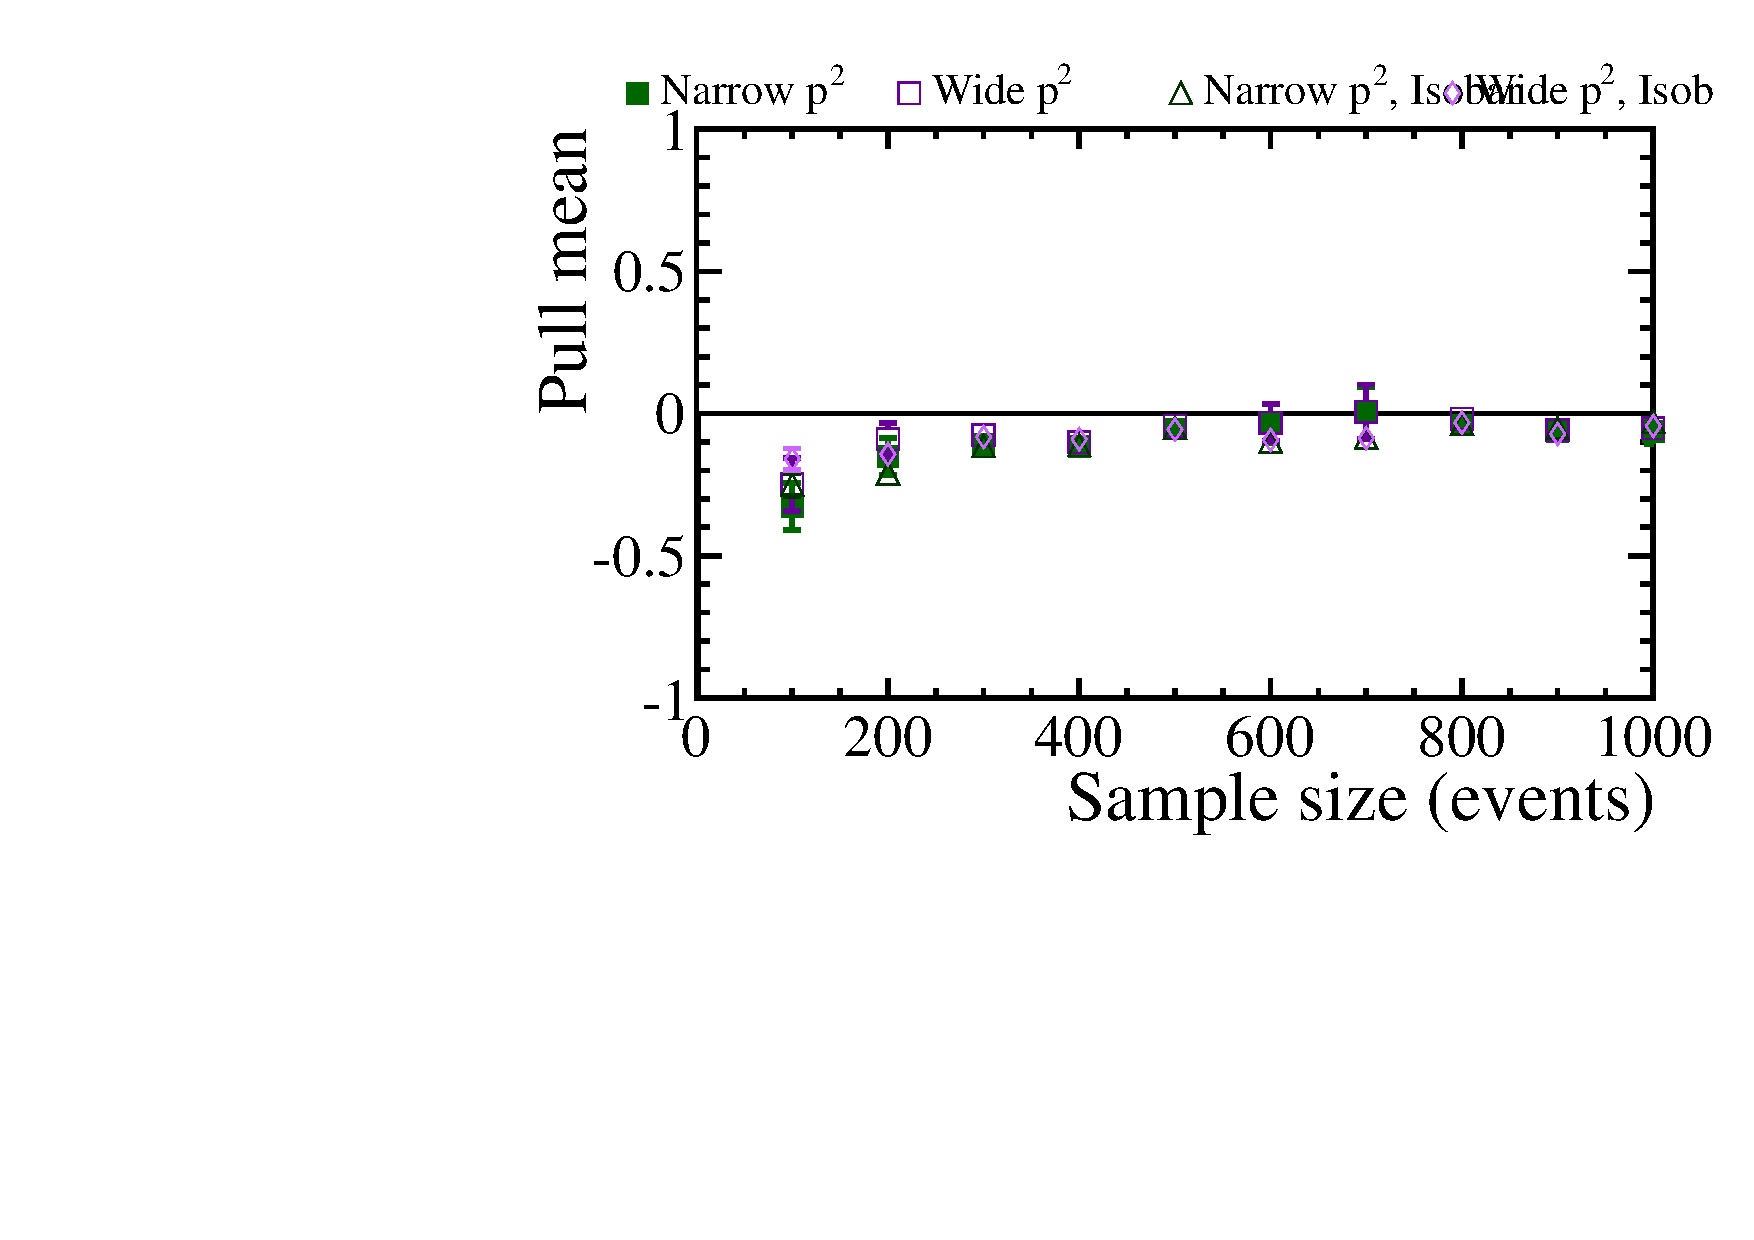
\includegraphics[width=0.48\textwidth]{chapter6/figs/fit_result_combo_ds_isobar_afb_mean.pdf}}
\subfigure[\FL]{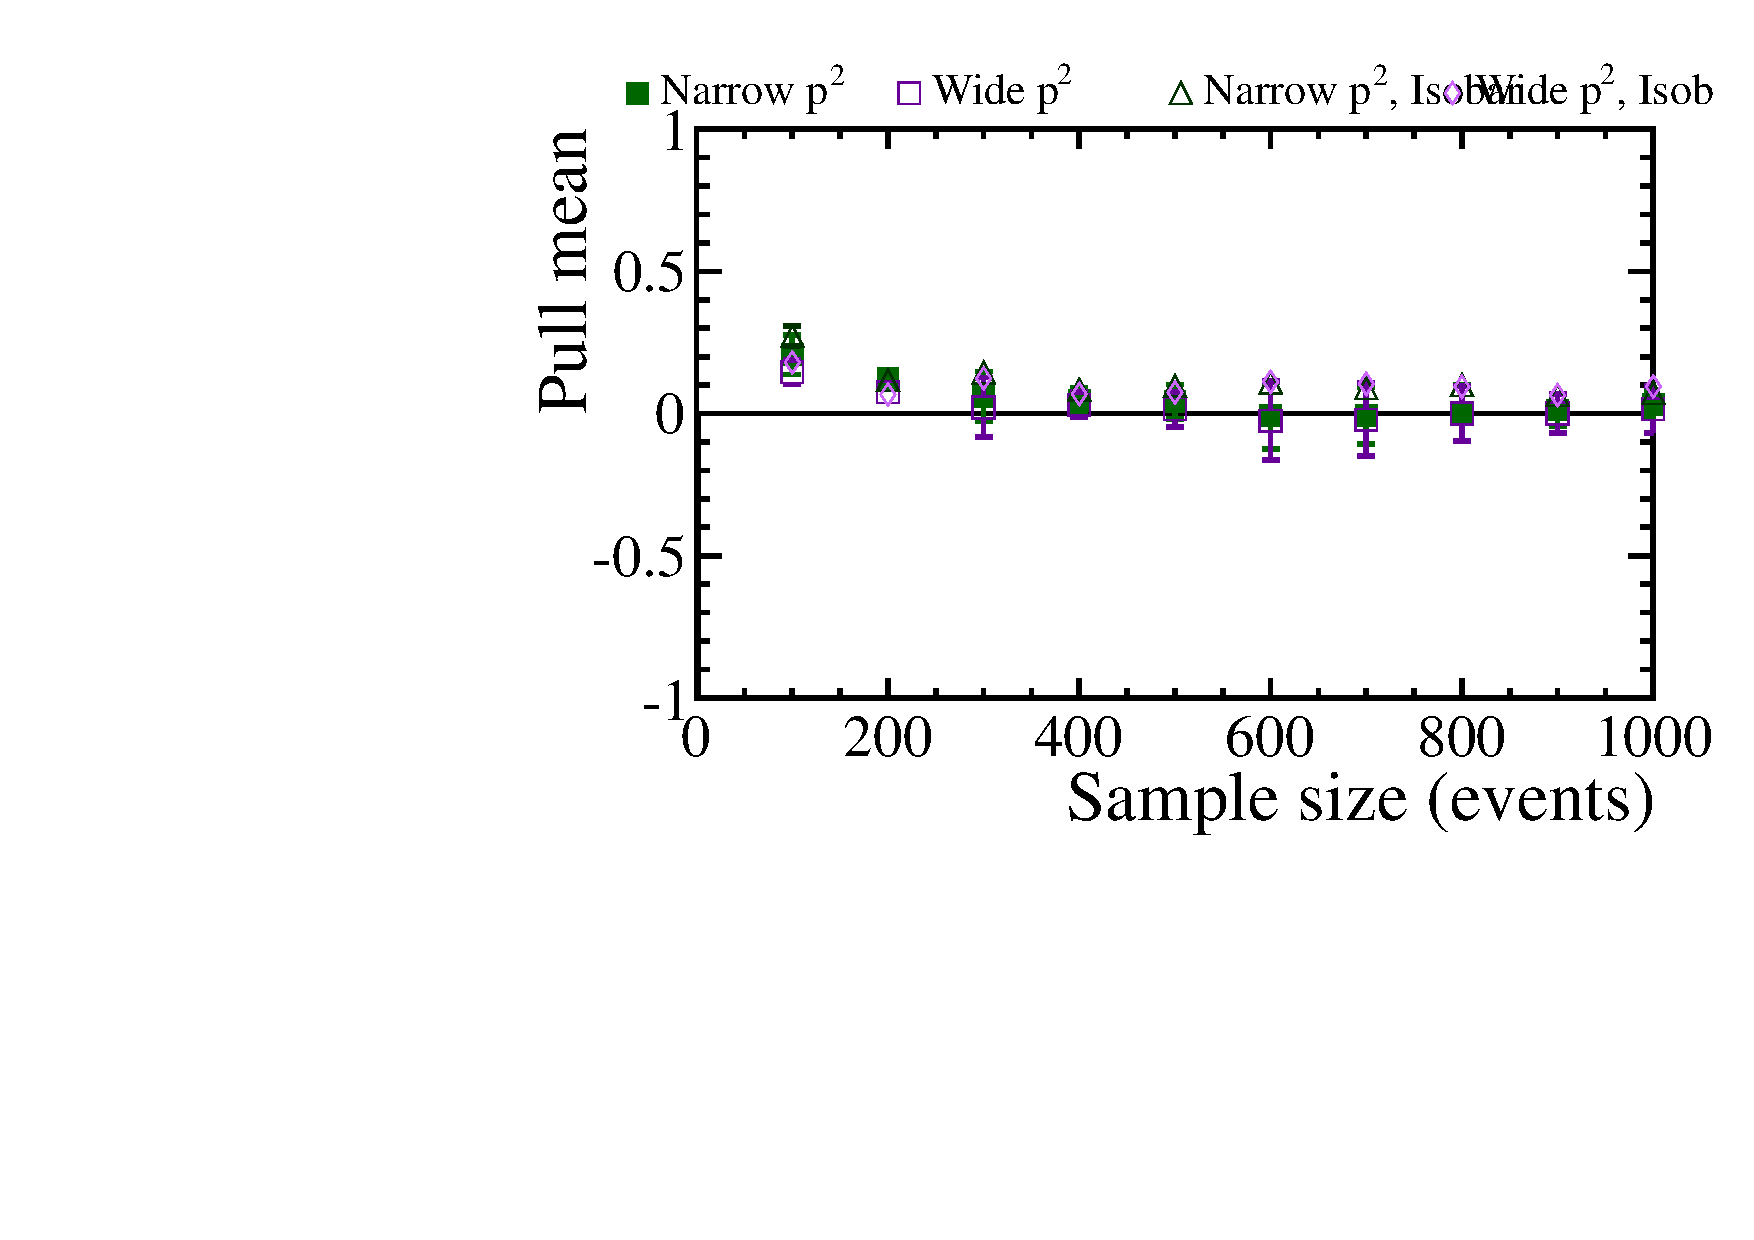
\includegraphics[width=0.48\textwidth]{chapter6/figs/fit_result_combo_ds_isobar_fl_mean.pdf}}
\subfigure[\AT2 ]{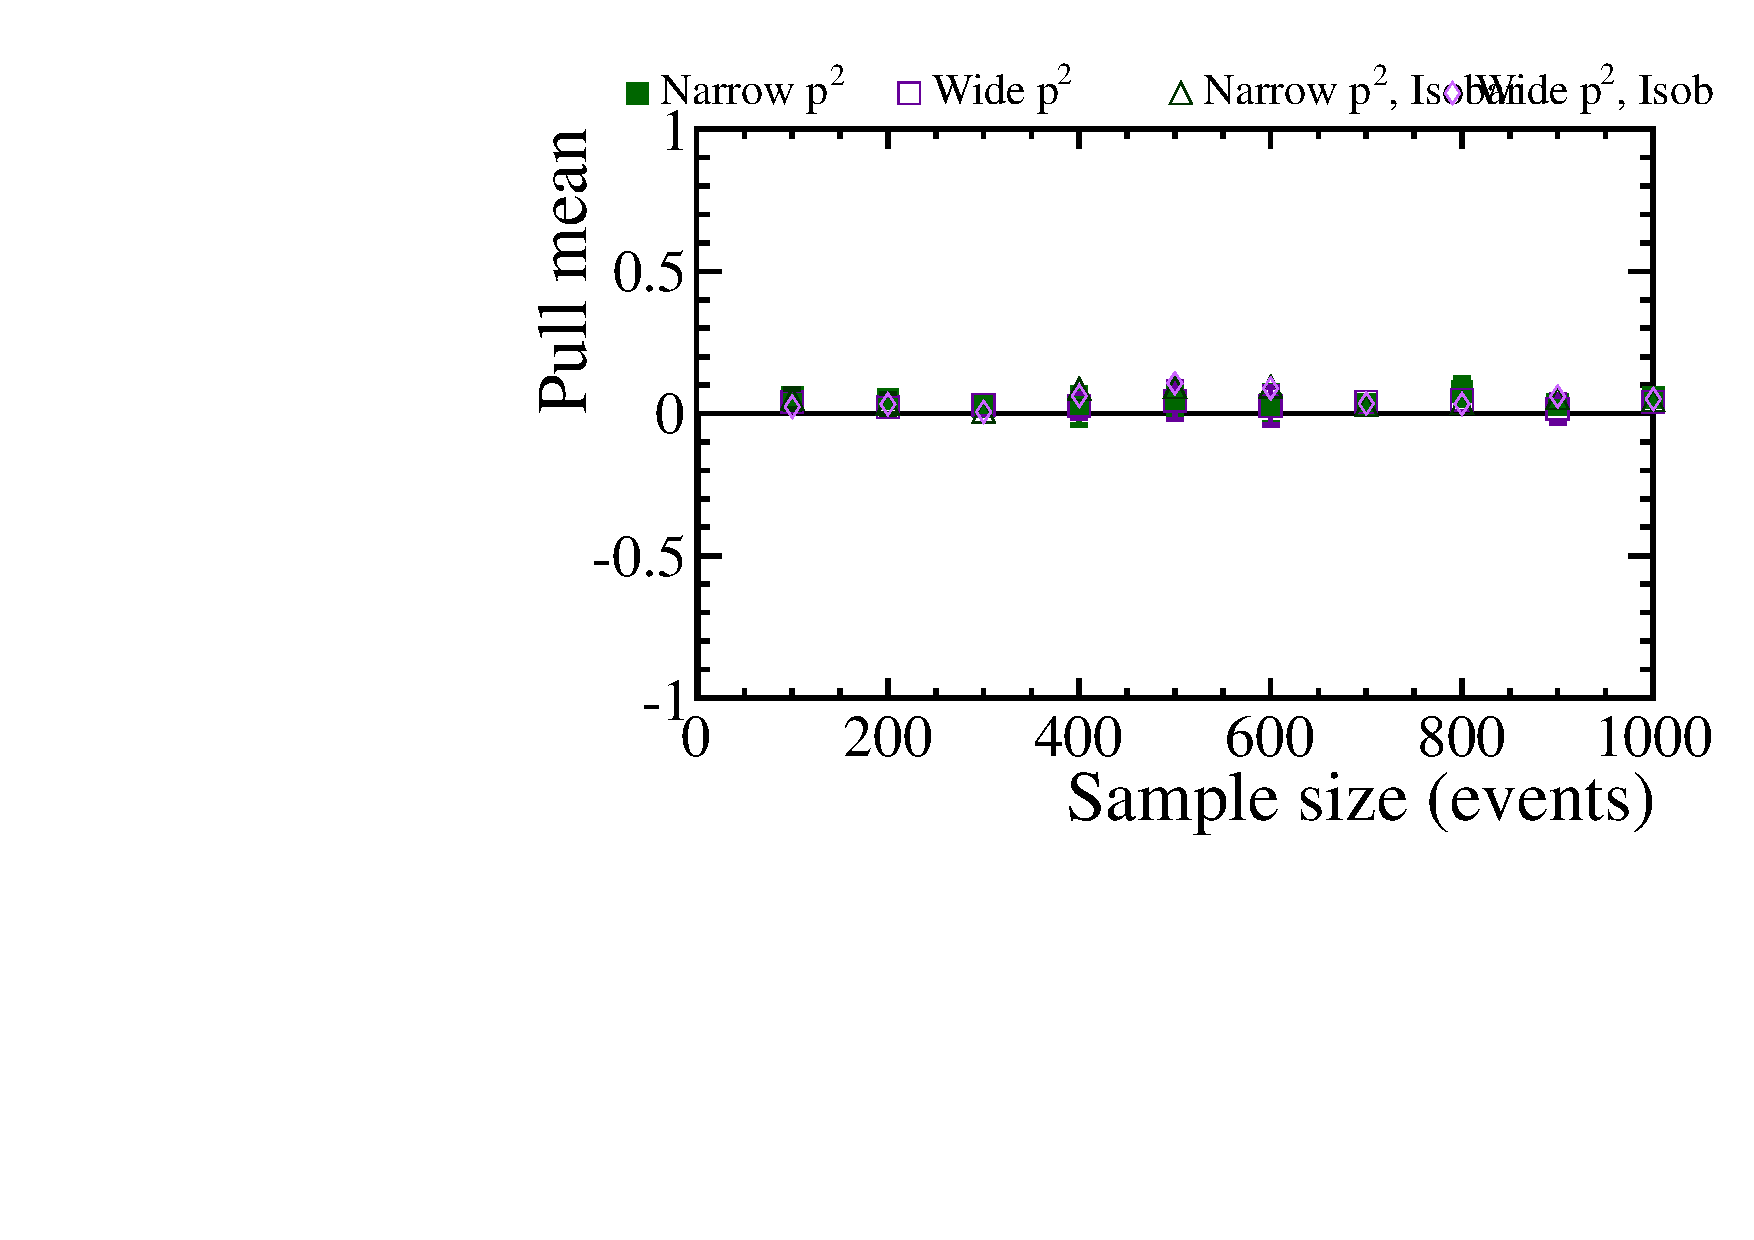
\includegraphics[width=0.48\textwidth]{chapter6/figs/fit_result_combo_ds_isobar_at2_mean.pdf}}
\subfigure[\AIm]{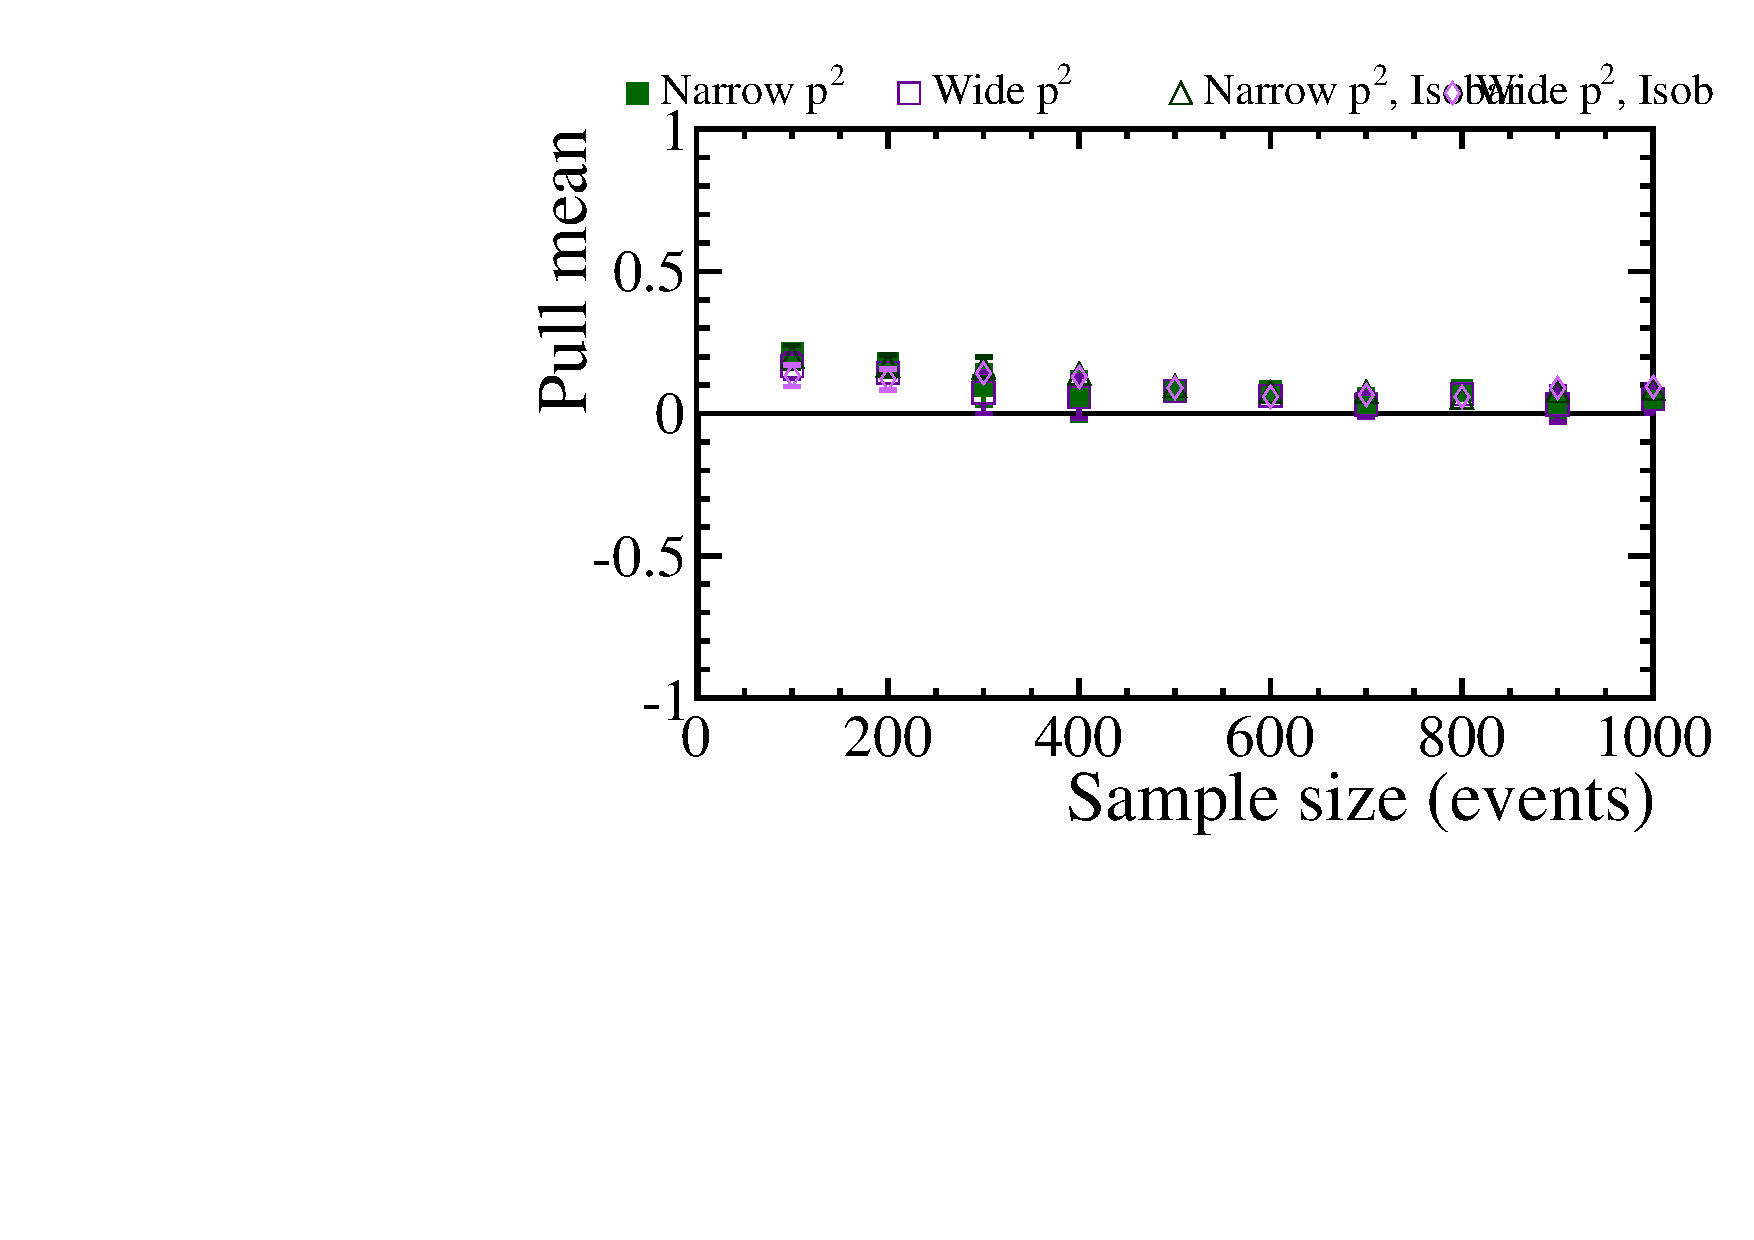
\includegraphics[width=0.48\textwidth]{chapter6/figs/fit_result_combo_ds_isobar_aim_mean.pdf}}
\caption[ Pull mean for the three different  
methods to incorporate the S-wave and when the S-wave 
is ignored.      ]
{Pull mean for the three different  
methods to incorporate the S-wave and when the S-wave 
is ignored. 
The S-wave has been generated using an isobar model.
 There is a slight shift when the S-wave is 
included for datasets of less than 200 events but this is removed from  all the observables 
when the S-wave is included in the fit 
for datasets of over 500 events. ~\label{fig:combods:isobar}}
\end{figure}
From this it is possible to see that the results obtained in Sec.~\ref{sec:swave:measurement} are compatible 
with the results where the events are generated with a different model for the \kpi continuum.
